\documentclass[11pt,a4paper]{article}

\usepackage[margin=2.3cm]{geometry}
\linespread{1.0}
\makeatletter
\renewcommand\section{\@startsection{section}{1}{\z@}{8pt plus 2pt}{5pt}{\normalfont\large\bfseries}}
\renewcommand\subsection{\@startsection{subsection}{2}{\z@}{6pt plus 2pt}{3pt}{\normalfont\normalsize\bfseries}}
\makeatother
\usepackage{enumitem}
\setlist{nosep,leftmargin=*}
\setlength{\textfloatsep}{6pt plus 2pt minus 2pt}
\setlength{\floatsep}{6pt plus 2pt minus 2pt}
\setlength{\intextsep}{6pt plus 2pt minus 2pt}
\usepackage[T1]{fontenc}
\usepackage[utf8]{inputenc}
\usepackage{mathptmx}
\usepackage{amsmath}
\usepackage{booktabs}
\usepackage{float}
\usepackage{graphicx}
\usepackage[hidelinks]{hyperref}
\graphicspath{{figures/}}

\title{Bayesian Network for Insider-Related\\Cyber Security Risk}
\author{Jan Ruijgrok\\Open University of the Netherlands}
\date{%
  \ifcase\month\or
    January\or February\or March\or April\or May\or June\or
    July\or August\or September\or October\or November\or December\fi
  \space\number\year}

\begin{document}
\maketitle

\begin{abstract}
Security teams assessing insider threats face incomplete HR, access, and monitoring signals; shareable incident data are scarce. This report develops and evaluates a compact Bayesian network for malicious insider-related cyber security risk. Experts specify people, process, and technology links; the model updates incident probability as evidence arrives. We validate inference on expert scenarios and test structure learning and classification on synthetically generated cases. Low- and high-risk profiles separate clearly; structure recovery improves with more data but edge direction remains harder than connectivity; on small test sets no classifier clearly dominates. The work is a proof of concept for analyst prioritisation, not validation on live operations data.
\end{abstract}

\noindent\textbf{Keywords:}
insider threat; cyber security risk; Bayesian network; noisy-OR; structure learning; classification; ROC curve; People--Process--Technology.

\section*{Notation and symbols}

\begin{table}[H]
\centering
\footnotesize
\caption{Main mathematical symbols.}
\label{tab:symbols}
\begin{tabular}{@{}lp{10.5cm}@{}}
\toprule
Symbol & Meaning \\
\midrule
$I$ & InsiderThreatIncident (class) \\
$E$ & Observed evidence \\
$P(I{=}\text{yes}\mid E)$ & Target posterior incident probability \\
$q$, $p_i$ & Noisy-OR leak and inhibitions on the incident node \\
$n$, $N$ & Structure-learning subset size; synthetic pool ($N{=}2000$) \\
$AUC$, $\mathrm{F1}$ & Area under ROC curve; graph recovery score \\
\bottomrule
\end{tabular}
\end{table}

\begin{table}[H]
\centering
\scriptsize
\caption{Network variables (eight nodes).}
\label{tab:variables}
\begin{tabular}{@{}llp{4.8cm}@{}}
\toprule
Variable & States & Description \\
\midrule
JobDissatisfaction & low, medium, high & Employee dissatisfaction or frustration with work or the work environment. \\
SecurityAwareness & low, medium, high & Employee knowledge and awareness of security risks and safe behaviour. \\
PolicyCompliance & good, poor & Extent to which employees and processes adhere to security policy. \\
ConcerningBehaviour & no, yes & Observed behaviour suggesting possible malicious intent or misuse. \\
PrivilegedAccess & appropriate, excessive & Whether access rights are appropriate for the role or excessively granted. \\
TechnicalControls & weak, adequate & Strength of preventive and detective technical measures (logging, Data Loss Prevention, etc.). \\
MonitoringAlert & no, yes & Whether monitoring generated an alert from behavioural or technical signals. \\
InsiderThreatIncident & no, yes & Whether a malicious insider-related security incident occurred. \\
\bottomrule
\end{tabular}
\end{table}

\section{Introduction}
When a security team suspects an insider threat, HR may report low morale, IAM tools may flag excessive privileged access, and monitoring may raise alerts---yet it remains unclear how likely a real incident is.
Shareable insider-incident data are scarce \cite{chockalingam2017}, so models must combine expert judgement with partial observations rather than rely on large labelled breach corpora.
Bayesian Networks (BNs) encode such judgement as a directed graph. They update $P(I{=}\text{yes}\mid E)$ as evidence arrives, exposing \emph{which} factors raise risk rather than a single opaque score.
A flat classifier could rank cases. It would not, however, separate expert causal structure from fitted parameters or support transparent what-if queries when evidence changes.
Chockalingam et al.\ \cite{chockalingam2017} find that published cyber-security BNs are typically small and expert-parameterised. Most follow a People--Process--Technology structure, focus on malicious insiders, and rarely integrate insider--outsider models.
Earlier insider-threat BNs link dissatisfaction, behaviour, and access misuse to higher risk \cite{axelrad2013}.
Against that background we build and test a compact eight-node network (Tables~\ref{tab:symbols}--\ref{tab:variables}). Our goal is to assess whether such an expert-built model can help analysts prioritise cases when signals are only partly visible and shareable incident data are scarce. We hypothesise that a domain-informed causal network yields interpretable risk estimates and remains competitive with data-driven alternatives on synthetically generated cases. We therefore examine scenario inference from expert probabilities, structure recovery as training data grow, incident prediction against learned and simpler classifiers on a small unseen set, and whether a parsimonious incident parameterisation preserves rising risk when more warning signs are active.

\section{Methods}
\label{sec:methods}

\subsection{Setup}
Four steps: (1)~specify the DAG and CPTs by expert judgement and test by inference only; (2)~generate $N{=}2000$ synthetic cases from that BN because real insider logs are unavailable; (3)~run structure learning and classification on held-out subsets; (4)~compare noisy-OR with a fuller incident CPT.
For classification we draw Train/Test $=100/100$ cases from a 300-row pool, \textbf{stratified} on~$I$.
Learning experiments are deliberately circular---they measure recoverability of a known graph, not external validity.

\subsection{Network}
Roots capture dissatisfaction and security awareness; process compliance shapes access; people and technology indicators feed the incident node.
Causally, dissatisfaction may precede concerning behaviour; weak controls influence both incidents and alerts.
The incident CPT is a noisy-OR over three activators: concerning behaviour (yes), excessive privileged access, and weak technical controls.
Figure~\ref{fig:dag} summarises the structure.

\begin{figure}[H]
  \centering
  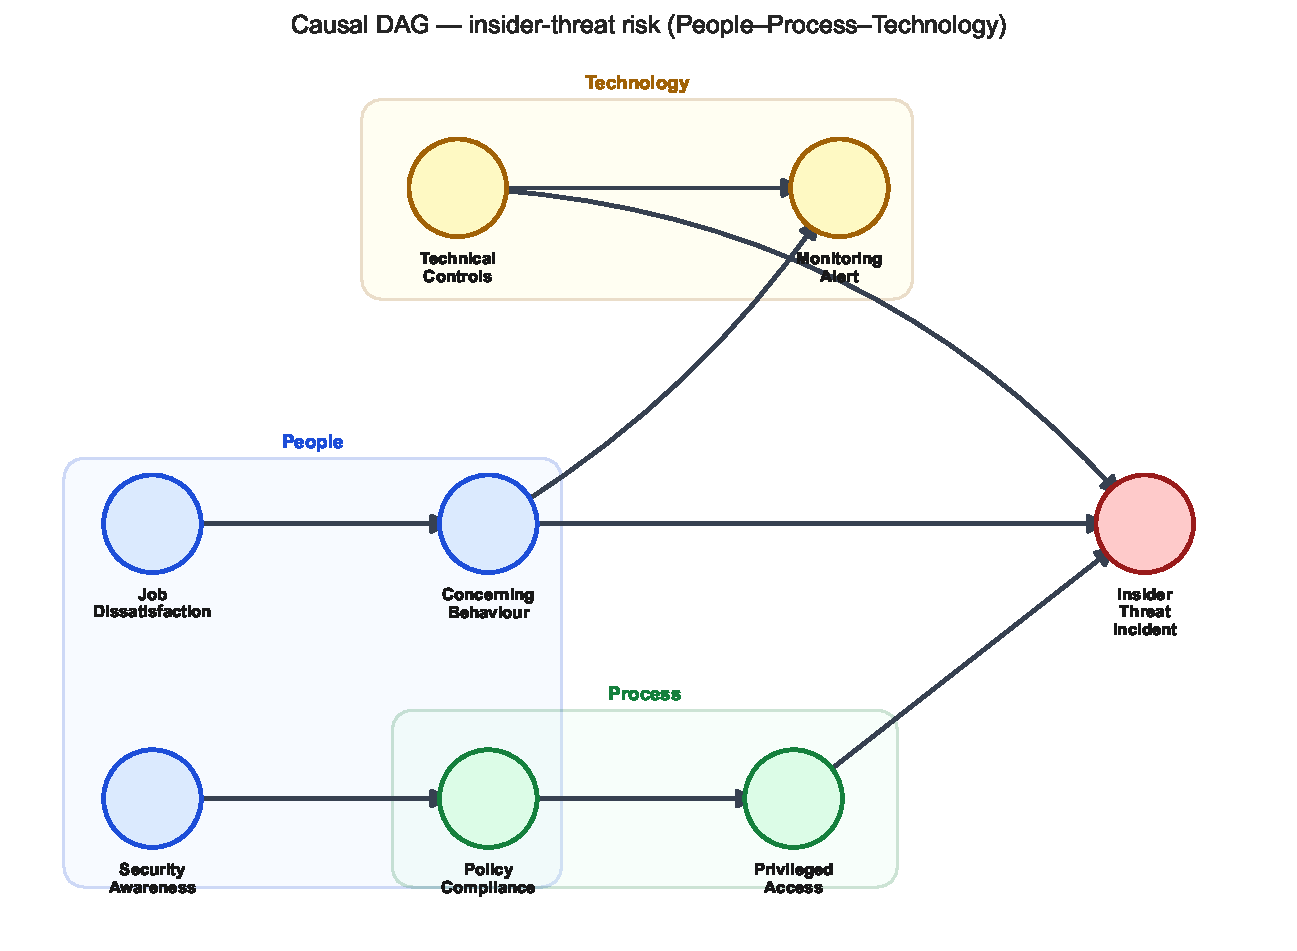
\includegraphics[width=0.95\linewidth]{fig01_dag.pdf}
  \caption{Causal DAG for insider-threat risk.}
  \label{fig:dag}
\end{figure}

\subsection{Learning}
For each $n\in\{100,500,1000\}$, learn structure and compare to the manual DAG (skeleton/directed $F_1$, Hamming distance).
For classification, we fix Train/Test $=100/100$ (stratified on~$I$): \emph{original} BN (expert DAG, CPTs on Train), \emph{learned} BN (Hill Climbing on Train), and \emph{naive Bayes} on the same variables. Primary metric: AUC. CPT fitting uses smoothing when 100 training rows leave parent configurations unobserved. Each experiment is repeated over 30 independent resamples (mean and 95\% percentile intervals). We compare four noisy-OR parameters with seven in a fuller logistic CPT, inspect $P(I{=}\text{yes})$ as activators turn on, and contrast Hill Climbing with MIIC for structure recovery. Domain-specific choices include a People--Process--Technology DAG, a noisy-OR incident node, and scenario evidence on the alert pathway.

\subsection{Data management}
All learning cases are simulated from the ground-truth BN ($N{=}2000$); no identifiable employee records were collected.

\section{Results}
\label{sec:results}

\subsection{Inference validation}
With the expert DAG and CPTs fixed, inference propagates evidence only. Table~\ref{tab:scenarios} and Figure~\ref{fig:scenarios} list five evidence profiles: high risk more than doubles baseline $P(I{=}\text{yes})$ ($0.74$ vs.\ $0.33$); low risk falls to $0.06$; an alert without a full pathway stays below baseline ($0.19$), consistent with the DAG. Dissatisfaction alone raises risk moderately ($0.40$). Varying the noisy-OR leak ($q\in\{0.90,0.94,0.97\}$) preserves the ordering high-risk $>$ baseline $>$ low-risk.

\begin{table}[H]
\centering
\footnotesize
\setlength{\tabcolsep}{3pt}
\begin{tabular}{@{}p{2.1cm}p{5.6cm}r@{}}
\toprule
Scenario & Key evidence set & $P(I{=}\text{yes})$ \\
\midrule
Baseline & (none) & 0.334 \\
High risk & CB=yes, PA=excessive, TC=weak & 0.743 \\
Low risk & CB=no, PA=appropriate, TC=adequate & 0.060 \\
Alert, low incident & MA=yes, CB=no, TC=adequate & 0.192 \\
High dissatisfaction & JD=high & 0.403 \\
\bottomrule
\end{tabular}
\caption{Scenario inference. CB = concerning behaviour; PA = privileged access; TC = technical controls; MA = monitoring alert; JD = job dissatisfaction.}
\label{tab:scenarios}
\end{table}

\begin{figure}[H]
  \centering
  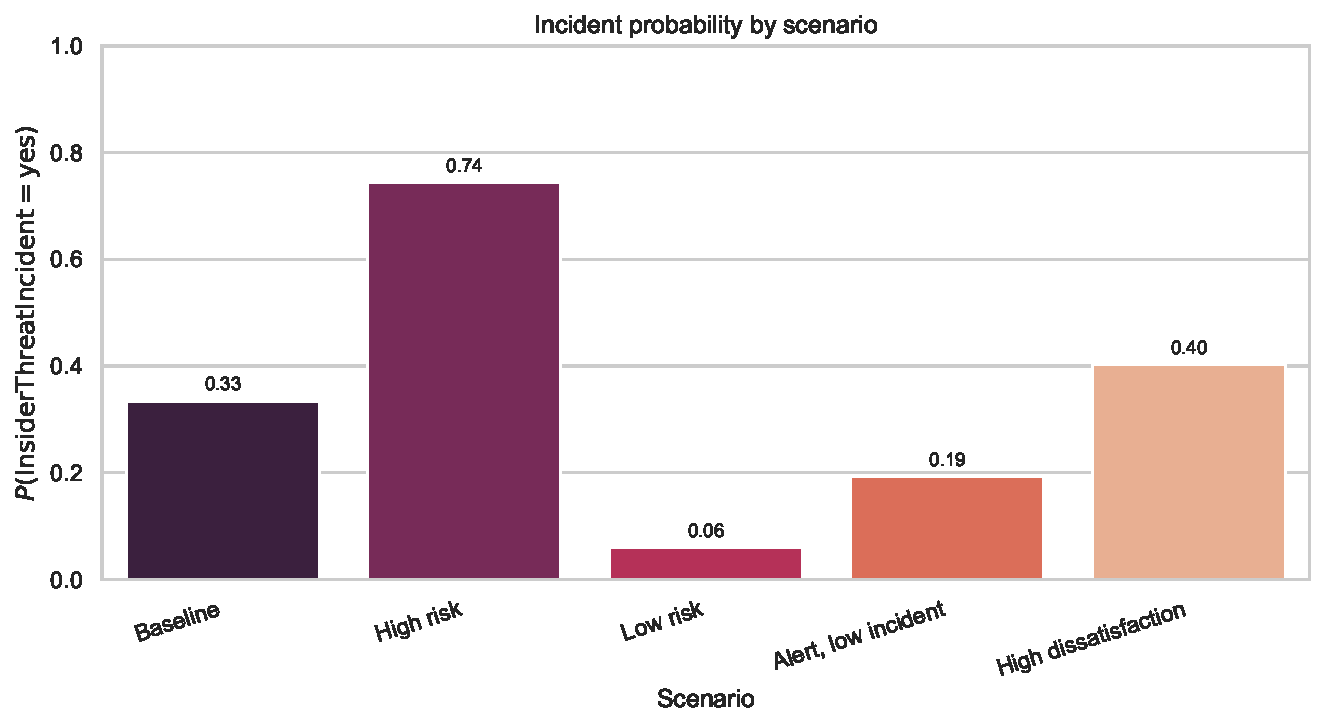
\includegraphics[width=0.72\linewidth]{fig02_scenarios.pdf}
  \caption{Incident probability by scenario.}
  \label{fig:scenarios}
\end{figure}

\subsection{Structure recovery}
Figure~\ref{fig:structure} and Tables~\ref{tab:structure-ref}--\ref{tab:structure} summarise learning from random subsets. Table~\ref{tab:structure-ref} gives one reference run (seed~42); Table~\ref{tab:structure} aggregates 30 resamples. Mean skeleton $F_1$ rises with~$n$; directed recovery stays harder for Hill Climbing, whereas MIIC reaches mean directed $F_1{\approx}0.96$ at $n{=}1000$.

\begin{table}[H]
\centering
\scriptsize
\setlength{\tabcolsep}{3pt}
\begin{tabular}{@{}rllccc@{}}
\toprule
$n$ & Algo. & Skeleton $F_1$ & Directed $F_1$ & Hamming \\
\midrule
100 & HC & 0.769 & 0.154 & 3 \\
100 & MIIC & 0.769 & 0.615 & 3 \\
500 & HC & 1.000 & 0.500 & 0 \\
500 & MIIC & 1.000 & 0.750 & 0 \\
1000 & HC & 0.889 & 0.111 & 2 \\
1000 & MIIC & 1.000 & 1.000 & 0 \\
\bottomrule
\end{tabular}
\caption{Reference structure-learning metrics (seed~42).}
\label{tab:structure-ref}
\end{table}

\begin{figure}[H]
  \centering
  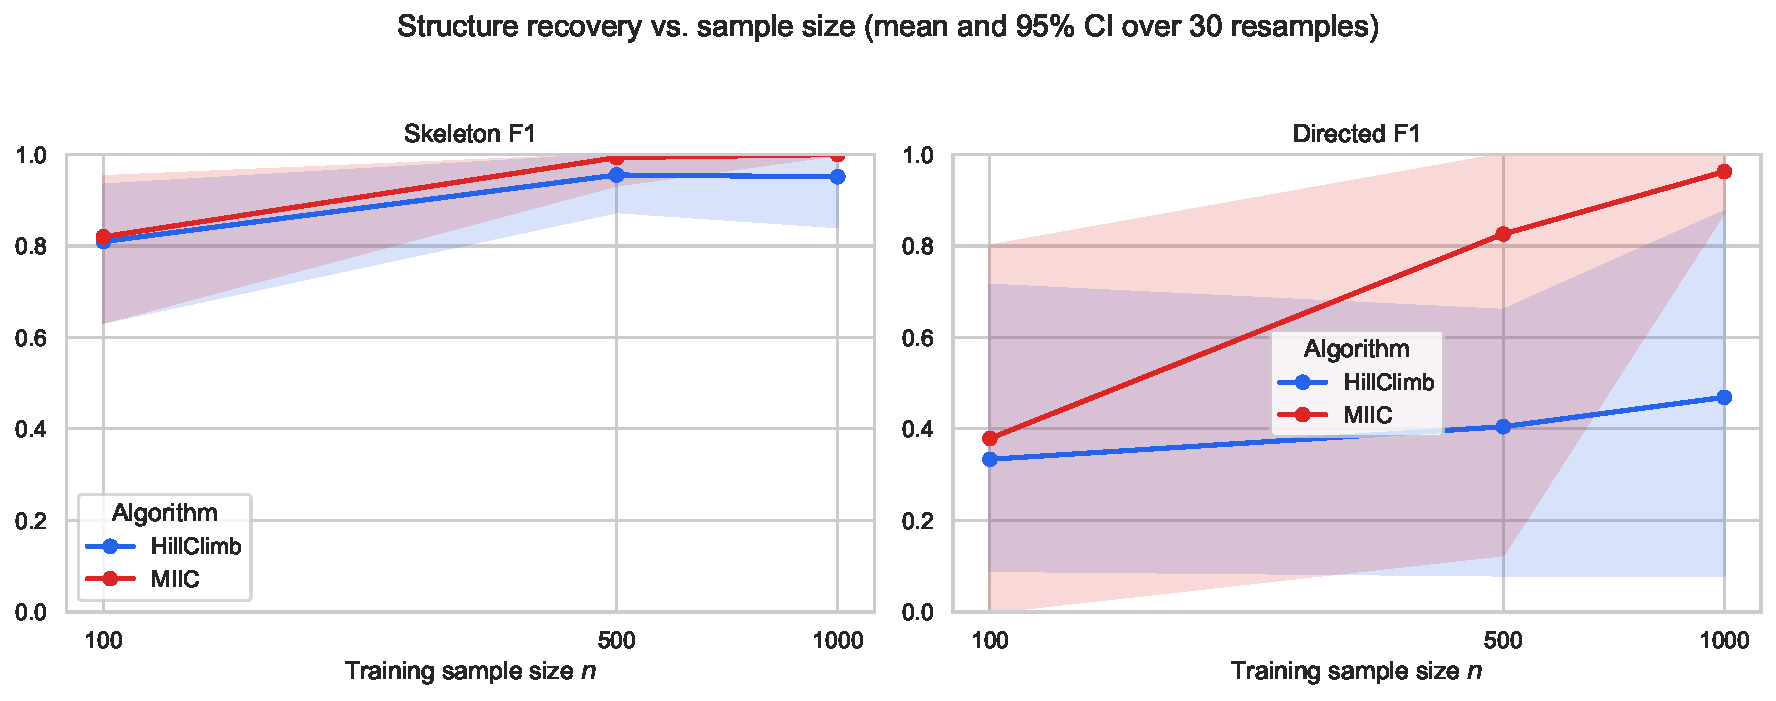
\includegraphics[width=0.88\linewidth]{fig03_structure_recovery.pdf}
  \caption{Structure recovery vs.\ $n$ (mean and 95\% CI over 30 resamples).}
  \label{fig:structure}
\end{figure}

\begin{table}[H]
\centering
\scriptsize
\setlength{\tabcolsep}{3pt}
\begin{tabular}{@{}rllcc@{}}
\toprule
$n$ & Algo. & Skeleton $F_1$ [95\% CI] & Directed $F_1$ [95\% CI] \\
\midrule
100 & HC & 0.788 [0.564, 0.933] & 0.367 [0.097, 0.714] \\
100 & MIIC & 0.807 [0.596, 0.933] & 0.390 [0.097, 0.703] \\
500 & HC & 0.961 [0.889, 1.000] & 0.506 [0.235, 0.875] \\
500 & MIIC & 0.978 [0.917, 1.000] & 0.797 [0.591, 1.000] \\
1000 & HC & 0.931 [0.811, 1.000] & 0.430 [0.000, 0.784] \\
1000 & MIIC & 0.996 [0.933, 1.000] & 0.962 [0.750, 1.000] \\
\bottomrule
\end{tabular}
\caption{Structure recovery stability (mean and 95\% CI over 30 resamples).}
\label{tab:structure}
\end{table}

Mean skeleton $F_1$ rises with~$n$ for both algorithms; MIIC reaches mean directed $F_1{\approx}0.96$ at $n{=}1000$ (Table~\ref{tab:structure}).

\subsection{Classification}
Reference and stability results appear in Tables~\ref{tab:classifiers}--\ref{tab:class-stability} and Figures~\ref{fig:roc}--\ref{fig:class-stability}. On one split, AUC ranges from 0.696 to 0.746; over 30 resamples the 95\% intervals overlap and no classifier clearly dominates.

\begin{table}[H]
\centering
\footnotesize
\begin{tabular}{lcc}
\toprule
Model & AUC & Accuracy \\
\midrule
Original BN & 0.746 & 0.69 \\
Learned BN (HC) & 0.696 & 0.66 \\
Naive Bayes & 0.743 & 0.70 \\
\bottomrule
\end{tabular}
\caption{Reference test performance on held-out cases.}
\label{tab:classifiers}
\end{table}

\begin{figure}[H]
  \centering
  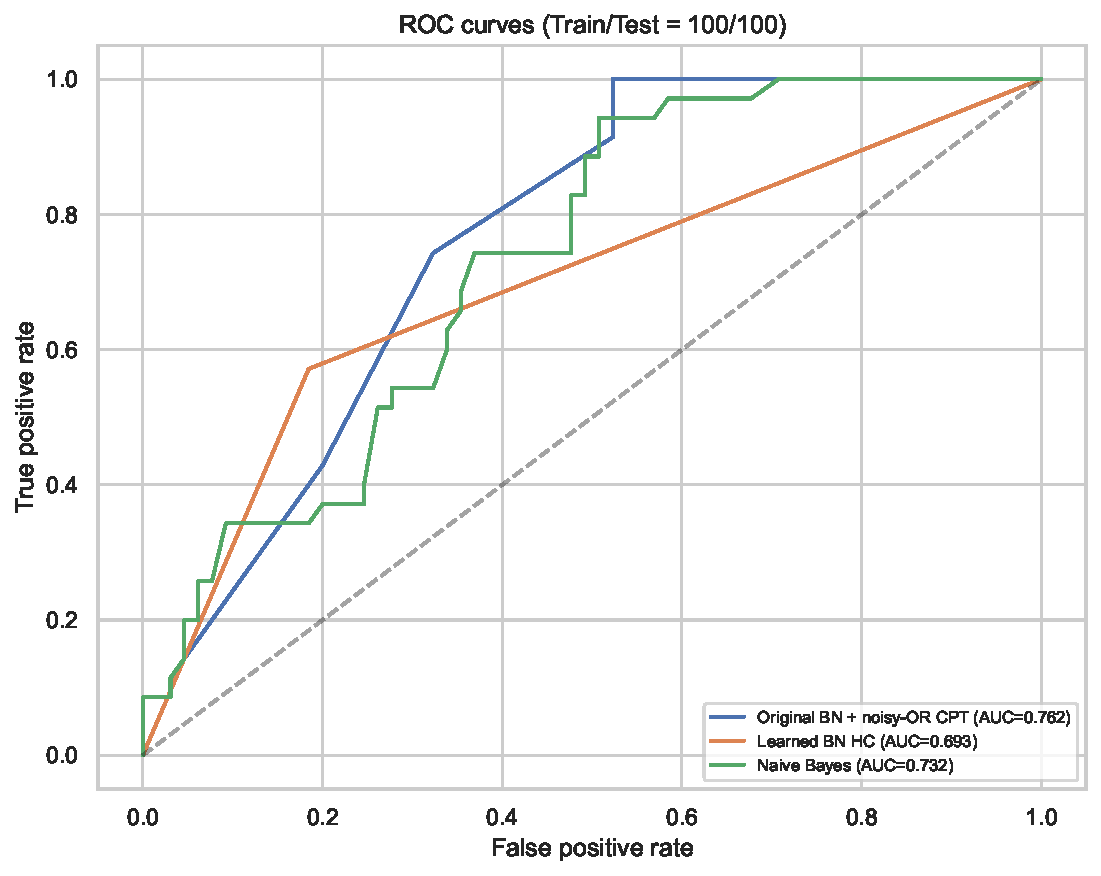
\includegraphics[width=0.65\linewidth]{fig04_roc.pdf}
  \caption{ROC curves on the reference split.}
  \label{fig:roc}
\end{figure}

\begin{table}[H]
\centering
\scriptsize
\setlength{\tabcolsep}{3pt}
\begin{tabular}{@{}lcc@{}}
\toprule
Model & AUC [95\% CI] & Accuracy [95\% CI] \\
\midrule
Original BN & 0.735 [0.627, 0.822] & 0.695 [0.609, 0.753] \\
Learned BN (HC) & 0.663 [0.496, 0.778] & 0.684 [0.580, 0.763] \\
Naive Bayes & 0.720 [0.585, 0.826] & 0.695 [0.605, 0.788] \\
\bottomrule
\end{tabular}
\caption{Classification stability over 30 resamples.}
\label{tab:class-stability}
\end{table}

\begin{figure}[H]
  \centering
  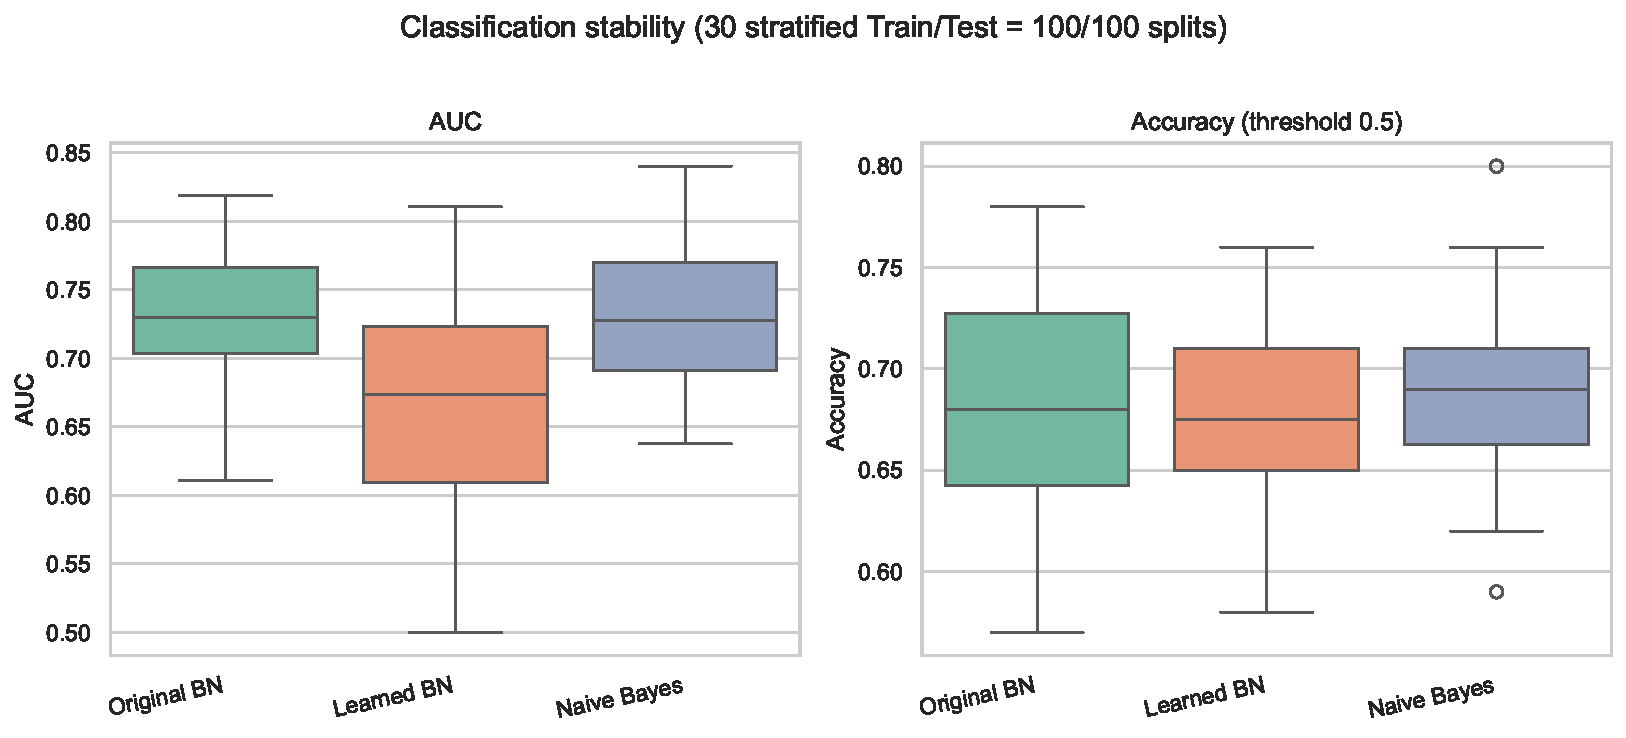
\includegraphics[width=0.70\linewidth]{fig06_classification_stability.pdf}
  \caption{Distribution of AUC and accuracy over 30 resamples.}
  \label{fig:class-stability}
\end{figure}

\subsection{Noisy-OR evaluation}
Noisy-OR uses four parameters instead of seven while preserving monotonic multi-cause risk (Figure~\ref{fig:noisyor}).

\begin{figure}[H]
  \centering
  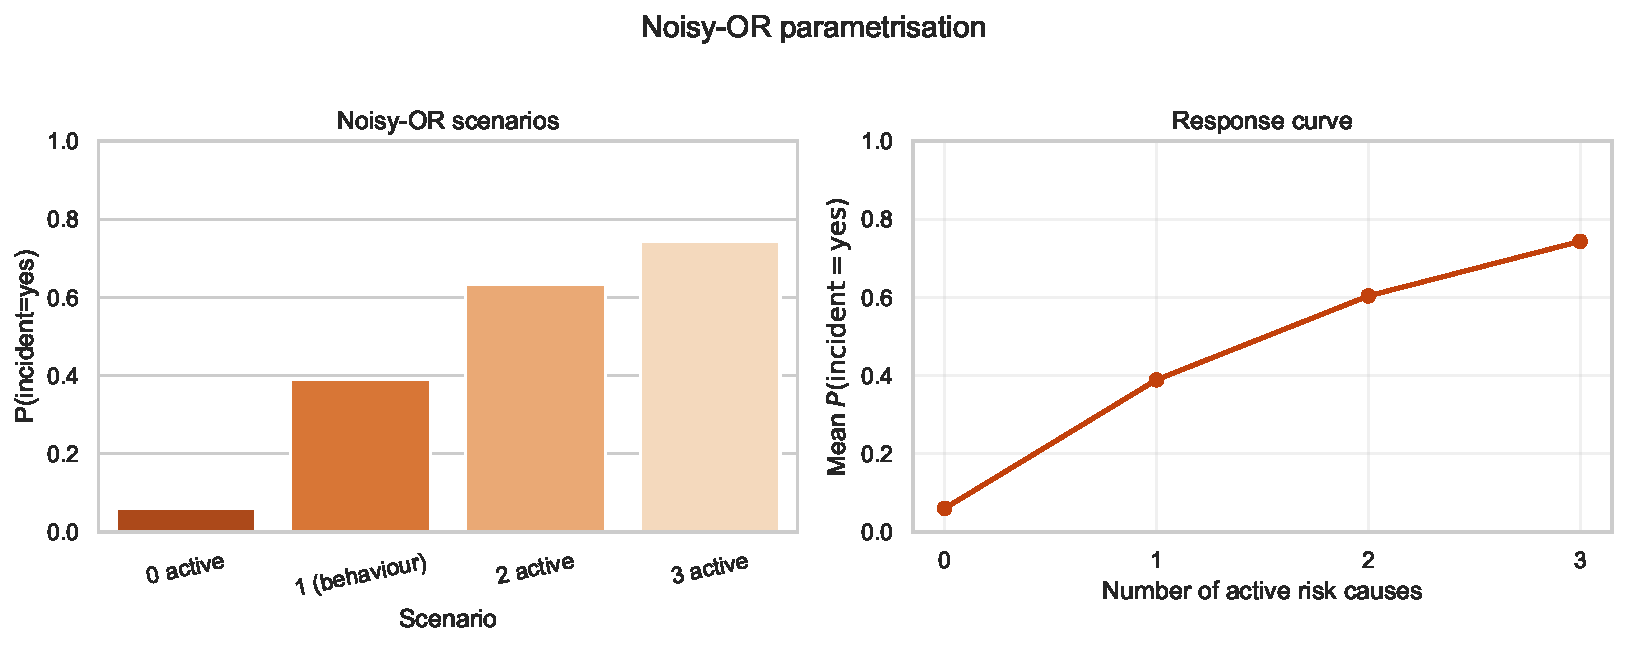
\includegraphics[width=0.72\linewidth]{fig05_noisy_or.pdf}
  \caption{Noisy-OR scenarios and response curve.}
  \label{fig:noisyor}
\end{figure}

\section{Conclusions and discussion}
\label{sec:conclusions}

\subsection{Summary of findings}
This study asked whether a compact, expert-built Bayesian Network can support insider-threat prioritisation when real incident data are scarce. The results suggest a qualified yes. Scenario inference produced stable, interpretable risk estimates; high- and low-risk profiles separated clearly. On synthetic data, skeleton recovery improved with sample size; directed recovery stayed harder for Hill Climbing while MIIC reached mean directed $F_1{\approx}0.95$ at $n{=}1000$. Classification intervals overlapped across models. Noisy-OR offered a parsimonious incident parameterisation with monotonic multi-cause risk.

\subsection{Limitations}
The evaluation is inward-looking: simulated learning data measure recoverability of a known graph, not external validity; CPTs reflect expert judgement, not operational calibration. The scope is a static malicious-insider People--Process--Technology graph \cite{chockalingam2017}; temporal HR and alert dynamics are not modelled. Small train and test sets ($n{=}100$ each) widen intervals: overlapping 95\% AUC bands (e.g.\ original BN $0.735$ vs.\ naive Bayes $0.720$) do not support definitive classifier ranking.

\subsection{Implications and future work}
Expert causal structure explains \emph{why} risk rises and remains competitive on average with learned alternatives. The pipeline is a proof of concept, not validation on live security-operations data; deployment would require human review and auditability. A realistic next step is to map operational feeds to the eight nodes, preregister elicitation and evaluation, document CPT workshops with sensitivity analysis, and trial analyst-facing scores with mandatory human review.

\noindent\textbf{Data and code availability.}
All analysis code, the reproducible Jupyter notebook, and exported figures are at \href{https://github.com/jruijgrok141/insider-threat-bayesian-network}{github.com/jruijgrok141/insider-threat-bayesian-network} (MIT license). Tables in \S\ref{sec:results} match \texttt{report/figures/*.csv} from \texttt{export\_figures.py} and pinned synthetic data; no identifiable employee records were used.

\clearpage
\bibliographystyle{plain}
\begin{thebibliography}{2}
\bibitem{chockalingam2017}
S.~Chockalingam, W.~Pieters, A.~Herdeiro Teixeira, and P.~van Gelder (2017).
Bayesian network models in cyber security: A systematic review.
In \emph{Proc.\ NordSec 2017} (LNCS 10674, pp.\ 105--122).
Springer. \url{https://doi.org/10.1007/978-3-319-70290-2_7}
\bibitem{axelrad2013}
E.~T. Axelrad, P.~J. Sticha, O.~Brdiczka, and J.~Shen (2013).
A Bayesian network model for predicting insider threats.
In \emph{IEEE Security and Privacy Workshops}, pp.\ 82--89.
\end{thebibliography}

\end{document}
